\begin{frame}{Introduction $\rightarrow$ 2 Frequency dependent fitness}

    \begin{itemize}    
        \item Game theory.
        \item $OncoSimulR$ model $\rightarrow$ the fitness of a subpopulation will depend on the relative abundance of the different subpopulations.
        \item The fitness of each subpopulation is defined as an arbitrary function of the genetic interactions between multiple genes.       
    \end{itemize}
    
\end{frame}

\begin{frame}{Introduction $\rightarrow$ Effects on fitness}

    \begin{itemize}
        \item $allFitnessEffects$ function:
        \begin{itemize}
            \item $genoFitness$ = dataframe
            \begin{itemize}
                \item First column: genotypes.
                \item Second column: expressions for the functions that relate fitness to frequencies of other genotypes.
            \end{itemize}
            \item $frequencyDependentFitness$ = TRUE
            \item $frequencyType$ = “rel” or $frequencyType$ = “abs”
            \item $spPopSizes$
        \end{itemize}        
    \end{itemize}

\end{frame}

\begin{frame}{Introduction $\rightarrow$ Assess fitness}

    \begin{itemize}
        \item $evalGenotype$ function:
        \begin{itemize}
            \item $fitnessEffects$ = $allFitnessEffects$ object
            \item $genotype$
        \end{itemize}
        \item $evalAllGenotypes$ function:
        \begin{itemize}
            \item $fitnessEffects$ = $allFitnessEffects$ object
        \end{itemize}
    \end{itemize}
    
\end{frame}

\begin{frame}{Introduction $\rightarrow$ Perform simulations}

    \begin{itemize}
        \item $oncoSimulIndiv$ and $oncoSimulPop$ functions.
    \end{itemize}
    \begin{columns}
        \begin{column}{0.5\textwidth}
            \begin{figure}[t]
                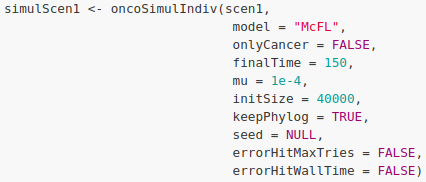
\includegraphics[width=0.9\linewidth]{img/oncoSimulIndiv.png}
            \end{figure}
        \end{column}
        \begin{column}{0.5\textwidth}
            \begin{figure}[t]
                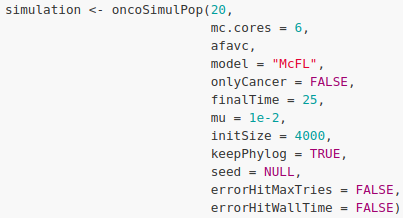
\includegraphics[width=0.9\linewidth]{img/oncoSimulPop.png}
            \end{figure}
        \end{column}
    \end{columns}
    
\end{frame}